\documentclass[times,usenatbib]{mn2e}
\RequirePackage{graphicx}
\RequirePackage{subfigure}
\RequirePackage{rotating}

\newcommand{\hiir}{H~{\scshape ii}~region}
\newcommand{\hiirs}{H~{\scshape ii}~regions}
\newcommand{\um}{$\mu$m}
\newcommand{\degree}{^{\circ}}
\newcommand{\apj}{ApJ}
\newcommand{\apjs}{ApJS}
\newcommand{\apjl}{ApJL}
\newcommand{\aj}{AJ}
\newcommand{\mnras}{MNRAS}
\newcommand{\pasp}{PASP}
\newcommand{\aap}{A\&A}

\title[Galaxies in the ZoA]{The Milky Way Project: Galaxies in the Zone of Avoidance\footnote{This publication has been made possible by the participation of more than 40,000 volunteers.}}

\author[Simpson et al.]
{\parbox{\textwidth}{R. J. Simpson$^{1}$\thanks{Email: robert.simpson@astro.ox.ac.uk},
K. Clements$^{2}$,
A. Gazzard$^{3}$,
B. Simmons$^{1}$,
C. J. Lintott$^{1}$}\vspace{0.8cm}\\
\parbox{\textwidth}{
$^{1}$Oxford Astrophysics, Denys Wilkinson Building, Keble Road, Oxford, OX1 3RH, UK \\
$^{2}$Wheatley School, Oxford, UK \\
$^{2}$A. N. Other School, Oxford, UK }}

\date{Draft form \today .}

\pagerange{000--000}

\begin{document}

\label{firstpage}

\maketitle

\begin{abstract}

We report the discovery of 33 previously unknown galaxies in the Zone of Avoidance. We also present a method for identifying galaxies through data gathered from the citizen science website `The Milky Way Project'. 43 candidate galaxies are identified through correlation of markings from volunteers, inspecting Spitzer GLIMPSE and MIPSGAL survey data on `The Milky Way Project' website. The characteristics of these candidate, such as their locations, spectral energy distributions and redshift velocities are used to confirm whether they are galaxies. The magnitudes and integrated flux of the candidates are calculated in GLIMPSE bands 3.6$\mu$m, 4.5$\mu$m, 5.8$\mu$m and 8.0$\mu$m, and MIPSGAL band 24$\mu$m. The velocities of these 33 newly uncovered galaxies appear to correlate with the velocities of over-densities in the large-scale structure, at very low Galactic latitudes either side of the Zone of Avoidance. Our findings therefore suggest that the large-scale structure continues throughout the Zone of Avoidance, and highlight the potential for many more galaxies to be found in far-infrared survey data.

\end{abstract}
\begin{keywords}
H II regions -- infrared: ISM  -- ISM: dust -- stars: formation
\end{keywords}

\section{Introduction}

The Zone of Avoidance (ZoA) remains a literal gap in our knoweldge of the large-scale structure of galaxies in the universe, and prevents us from determining the dynamics of our local Universe. Redshift surveys have steadily improved our knowledge of the large-scale structure above and below the ZoA (e.g., CfA Redshift Survey, Geller \& Huchra 1989; 2dF Redshift Survey, Colless 1999; Las Campanas Redshift Survey, Shectman et al. 1996). However, the precise way the coherent structures of the two halves connect remains largely unknown, and currently needs to be simulated -- a problem highlighted by the case of the `Great Attractor' at Galactic longitude l~320$^{\circ}$ and latitude b~0$^{\circ}$ (Kolatt et al. 1995).

The Spizter GLIMPSE and MIPSGAL surveys (Benjamin et. al. 2003, Carey et al. 2008), surveyed the Galactic midplane in a multitude of infrared wavelengths. These landmark surveys provided the opportunity to occaisonally see through the obscuring material of our own Galaxy. One of the first extragalactic results from GLIMPSE/MIPSGAL was the \citet{Jarrett+07} discovery of two galaxies obvserved through our Galaxy, toward of the Great Attractor. Following this \citet{Marleau+08} demonstrated further the discovery potential of Spitzer in the ZoA by revealing 25 further highly-obscured galaxies.

\section{The Milky Way Project}
\label{mwp-desc}

The Milky Way Project \citep[MWP,][]{Simpson+12} is the ninth online citizen science project created using the Zooniverse\footnote{http://www.zooniverse.org} platform \citep{2011MNRAS.412.1309S}. The Zooniverse platform supports the activities of all Zooniverse citizen science projects. Built originally for Galaxy Zoo 2 this software, and successive versions of it, have now been used by more than 20 different projects across a range of research disciplines. The Zooniverse toolset is designed primarily as a way to of serving a large collection of `assets' (for example, images or video) to a user interface, and collecting back user-generated interactions with these assets.

Galaxy Zoo \citep{Lintott+08, Lintott+11} and the larger suite of Zooniverse projects have successfully built a large community of volunteers\footnote{Over 750,000 registered volunteers at time of writing.} eager to participate in scientific activities. The Zooniverse has shown that enlisting these `citizen scientists' via the internet is a powerful way to analyze large amounts of data. Human brains excel at pattern recognition tasks, and most people will reach a level of accuracy as high as any expert after a brief introduction. By enlisting citizen scientists, researchers can extend visual classification to large samples of images, having each image examined by a large number of independent classifiers. This allows researchers to tap into the `wisdom of the crowd' effect where the consensus of a group of non-experts is often more accurate than the testimony of a single expert.

Another advantage of enlisting human classifiers is their ability to recognize unusual objects (e.g. galaxies, star clusters, dark clouds in the MWP) which computer search algorithms  may be unable to spot. This has been shown by the serendipitous discovery of Hanny's Voorwerp \citep{2009MNRAS.399..129L} and the case of the Galaxy Zoo `Green Peas' \citep{2009MNRAS.399.1191C}. Spitzer GLIMPSE data is ideally suited to classification by citizen scientists as the amount of data is large and the images contain complex, overlapping structures that are extremely difficult to disentangle using automated algorithms.

\begin{figure}
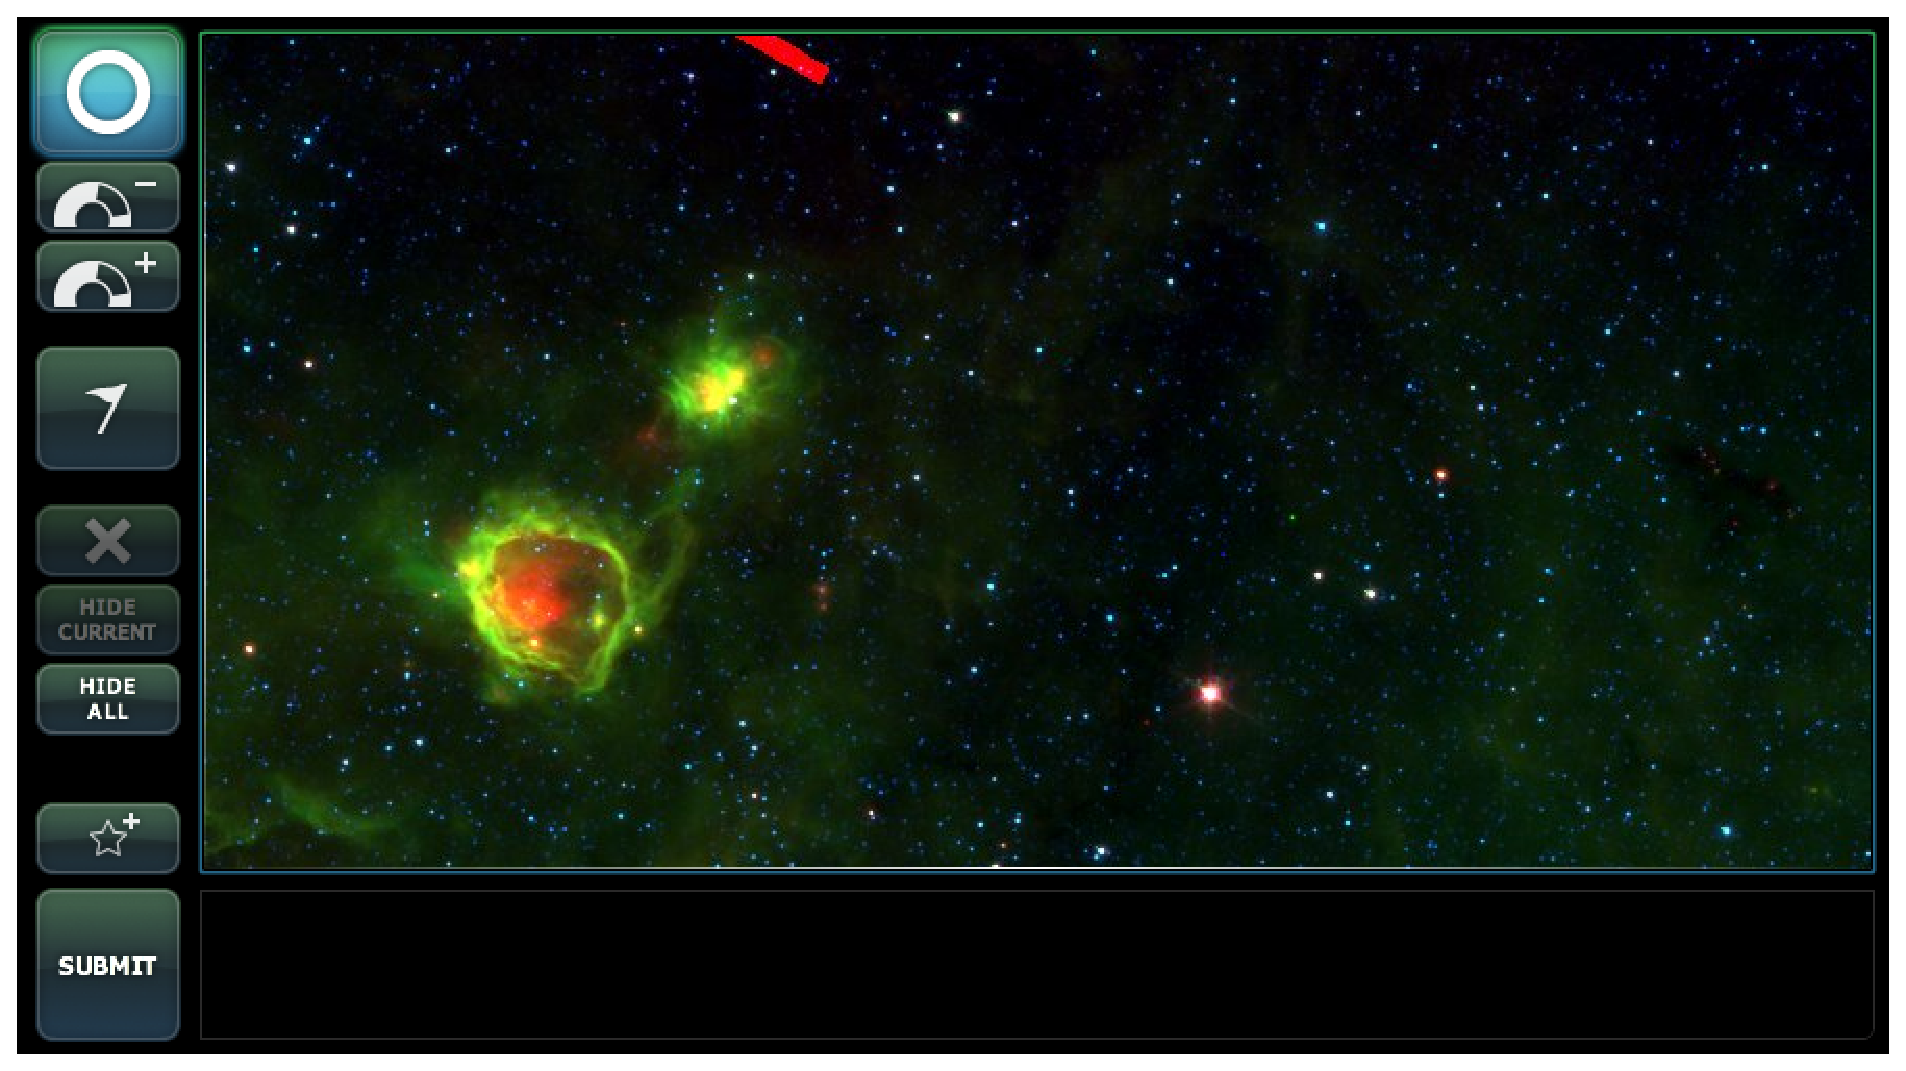
\includegraphics[width=0.48\textwidth]{./figures/user-interface.eps}
\caption{Screenshot of the Milky Way Project user interface. Colour figure available online.}
\label{user-interface}
\end{figure}

The assets in the MWP are multiband, false-colour JPEG images, created by gridding the {\it Spitzer} GLIMPSE and MIPSGAL mosaics into smaller images at three different zoom levels. The highest zoom level provides users with tiles of 0.3$^{\circ}\times$0.15$^{\circ}$, and at a resolution of 800$\times$400 pixels these tiles nearly reproduce the $1.2''$ pixel scale of the GLIMPSE survey images. Larger tile sizes of 0.75$^{\circ}\times$0.375$^{\circ}$ and 1.5$^{\circ}\times$0.75$^{\circ}$ were also generated. The tiles were plotted in an overlapping grid to allow all parts of the inner Galactic plane ($|l|\le 65\degree$, $|b|\le 1\degree$) to be viewed by the MWP users, at all zoom levels. To provide an optimal representation of the dynamic range within each tile, each of 3 single-band images was independently scaled to a square-root stretch function (with the faintest 5\% of image pixels clipped to black and the brightest 0.2\% clipped to white), assigned to a colour channel (red=24~\um, green=8.0~\um, blue=4.5~\um), and finally composited into a 3--colour image. The MIPSGAL 24~\um\ mosaics frequently saturate in regions of bright nebulosity, and saturated 24~\um\ pixels were set to maximum red to preserve the visual appeal of the images and to avoid presenting MWP users with saturation artefacts. The resulting composite images allow visual identification of both bright and faint features within a given image tile.

The MWP user interface (see Figure~\ref{user-interface}) was built using Flash, based upon the pre-existing Moon Zoo interface \citep{Joy+11}. Volunteers are primarily encouraged to draw ellipses onto the image to mark the locations of bubbles. A short, online tutorial shows how to use the tool, and examples of prominent bubbles are given\footnote{http://www.milkywayproject.org/tutorial}. As a secondary task, users can also mark rectangular areas of interest, which can be labelled as small bubbles, green knots, dark nebulae, star clusters, galaxies, fuzzy red objects or `other'. Examples of these are also given in a tutorial on the website, and it is the galaxies that will be dealt with in this study. Users can add as many annotations as they wish before submitting the image, at which point they are given another image for annotation. Each image's annotations are stored in a database as a classification, and users can see the images they have classified in a part of the site called `My Galaxy'. Users can only classify a given image once.

Volunteers are primarily asked to draw bubbles on the images, by placing elliptical annuli that match the structures they see in the data. They are also encouraged to mark other regions interest on an image, marking these are either star clusters, green knots, etc. Do do so, volunteers simply draw rectangles. Since these objects are secondary to the main bubble-finding task, the site was designed so that they should be simple and quick to mark. Simple rectangles allow us to record the positions and approximate sizes of any these other interesting objects.

\section{Catalogue construction}

The galaxy candidates presented here are derived from 30,529 galaxy annotations by volunteers on the MWP -- literally drawn as boxes on the sky at locations where they believed there \emph{might} be a galaxy. These boxes were gridded together on the basis of position and size, with a grid size equal to the smallest MWP annotation size of 20 pixels. The resulting list of 360 unique objects each have a calculated averaged position, height and width as well as a ratio of number-of-times-viewed to number-of-times-drawn by MWP volunteers (known as the `hit rate'). Only those objects drawn by at least three independent volunteers, and with a hit-rate of at least 10\%, were retained. This quality control step ensures that most spurious and unintentional drawings do not contaninate the reduced set and a similar measures is taken in \citet{Simpson+12}. The resultant XXXX objects were visually inspected. Any obvious outliers or misclassifications were removed (e.g. stars, diffraction spikes and small bubbles) and the final set of objects forms the list of 43 candidates shown in Table~\ref{candidate-catalogue}.

\begin{table*}
\begin{center}
\caption{Table of galaxy parameters, including galactic coordinates, corrected magnitudes for Spitzer IRAC bands 1, 2, 3 and 4, and the MIPS 24$\mu$m flux.}
\begin{tabular}{lccrrrrr}
\hline
ID & GLON & GLAT & 3.6$\mu$m & 4.5$\mu$m & 5.8$\mu$m & 8$\mu$m & 24$\mu$m \\
 & (deg) & (deg) & (mag) & (mag) & (mag) & (mag) & (mag) \\
\hline
 1 & 004.548483 & $-$0.781395 & 13.80 & 13.53 & 12.35 & 10.76 & 7.09 \\
 2 & 011.818667 & $-$0.025800 & 11.88 & 11.80 & 9.84 & 8.41 & 4.69 \\
 3 & 012.741267 & $-$0.000400 & 10.10 & 10.03 & 10.15 & 9.46 & 5.19 \\
 4 & 017.225237 & $-$0.584033 & 11.78 & 11.86 & 11.73 & 9.98 & 7.05 \\
 5 & 017.784417 & +0.034222 & 11.30 & 11.77 & 10.39 & 8.70 & 5.88 \\
 6 & 028.141688 & $-$0.192917 & 11.57 & 11.72 & 11.26 & 9.82 &  \\
 7 & 028.729475 & $-$0.539626 & 12.85 & 12.72 & 11.50 & 9.53 & 5.32 \\
 8 & 036.399831 & $-$0.466475 & 12.84 & 13.06 & 13.46 & 11.12 & 5.27 \\
 9 & 041.581565 & $-$0.884437 & 13.86 & 13.70 & 12.88 & 11.85 & 8.86 \\
10 & 042.908694 & $-$0.888909 & 14.23 & 13.88 & 13.45 & 11.27 & 8.13 \\
11 & 047.824267 & $-$0.390300 & 13.78 & 13.98 & 12.04 & 10.55 & 8.16 \\
12 & 048.707895 & +0.961547 & 13.25 & 13.38 & 12.60 & 11.42 & 7.93 \\
13 & 054.574569 & $-$0.511079 & 13.40 & 13.47 & 12.01 & 10.56 & 7.83 \\
14 & 054.657243 & $-$0.256119 & 12.94 & 12.83 & 11.52 & 9.89 & 6.62 \\
15 & 055.307833 & +0.810834 & 13.34 & 13.57 & 12.01 & 10.51 & 7.56 \\
16 & 057.474400 & $-$0.387300 & 13.44 & 13.28 & 12.11 & 10.52 & 7.14 \\
17 & 058.441232 & $-$0.470409 & 12.86 & 12.98 & 12.10 & 10.87 & 6.21 \\
18 & 059.217833 & +0.396467 & 14.39 & 14.78 & 15.41 & 12.04 & 8.35 \\
19 & 059.545904 & +0.776002 & 13.58 & 13.49 & 12.66 & 10.62 & 7.81 \\
20 & 061.350500 & $-$0.108500 & 13.98 & 14.02 & 13.44 & 11.62 & 8.66 \\
21 & 063.349203 & $-$0.768282 & 14.00 & 14.02 & 13.07 & 11.60 & 8.58 \\
22 & 299.362072 & +0.731691 & 14.22 & 14.80 & 15.95 & 12.44 & 9.98 \\
23 & 299.398377 & +0.888066 & 12.84 & 12.90 & 12.45 & 10.89 & 7.49 \\
24 & 302.037426 & $-$0.528374 & 13.12 & 12.96 & 11.62 & 9.65 & 6.68 \\
25 & 302.373292 & $-$0.023500 & 13.91 & 12.68 & 11.73 & 11.37 & 6.72 \\
26 & 306.681500 & +0.015125 & 10.86 & 10.80 & 10.47 & 9.82 & 6.56 \\
27 & 314.143892 & $-$0.682605 & 14.69 & 14.14 & 13.28 & 12.36 & 8.65 \\
28 & 316.873061 & $-$0.599138 & 12.03 & 12.04 & 10.99 & 9.64 & 6.47 \\
29 & 317.039057 & $-$0.497820 & 12.77 & 12.75 & 11.34 & 9.75 & 5.64 \\
30 & 318.527084 & +0.504229 & 13.02 & 12.89 & 12.20 & 10.60 & 7.08 \\
31 & 318.729619 & $-$0.097762 & 12.44 & 12.17 & 11.07 & 9.42 & 5.28 \\
32 & 321.402694 & +0.652191 & 11.52 & 11.27 & 9.84 & 8.33 & 5.12 \\
33 & 322.552422 & +0.815422 & 11.48 & 11.58 & 11.88 & 11.68 & 5.24 \\
34 & 324.323250 & +0.317000 & 13.48 & 13.39 & 12.26 & 10.96 & 7.90 \\
35 & 325.245517 & $-$0.799997 & 12.95 & 13.20 & 11.87 & 10.38 & 7.16 \\
36 & 333.445875 & +0.356375 & 12.10 & 11.86 & 10.60 & 9.06 & 7.23 \\
37 & 335.104583 & $-$0.066792 & 11.30 & 11.09 & 8.95 & 7.50 & 5.68 \\
38 & 335.517000 & $-$0.378042 & 11.02 & 11.05 & 10.38 & 9.12 & 5.24 \\
39 & 341.857467 & $-$0.842779 & 13.52 & 13.29 & 12.12 & 10.40 & 7.67 \\
40 & 350.457146 & $-$0.041708 & 13.45 & 13.46 & 14.21 & 13.08 & 7.47 \\
41 & 350.101407 & +0.389093 & 12.81 & 12.42 & 11.34 & 9.87 & 5.39 \\
42 & 357.148741 & $-$0.572130 & 13.61 & 13.47 & 12.53 & 10.89 & 6.83 \\
43 & 357.737833 & $-$0.092033 & 12.96 & 12.69 & 10.50 & 9.13 & 5.71 \\
\hline
\end{tabular}
\end{center}
\label{candidate-catalogue}
\end{table*}

\subsection{Aperture photometry}

Data from GLIMPSE (Benjamin et. al 2003) and MIPSGAL (Carey et. al. 2008) were downloaded from the NASA/IPAC Infrared Science Archive\footnote{http://irsa.ipac.caltech.edu} for each of the 43 candidate galaxies. These were in the form of cutouts in each of the four IRAC (Fazio et al. 2004) bands (3.6, 4.5, 5.8 and 8$\mu$m) and in the 24$\mu$m MIPS (Rieke et al. 2004) band. Three-colour IRAC composites for each candidate are shown in Figures~\ref{gallery2} and \ref{gallery2}. The original MWP images seen by users, are included in the appendix, alongside a selection of other data for each candidate.

The spectral energy disturbtion for each candidate was derived using photomtetric measurements from these data. The aperture size and position for each candidate were created using the visual controur of the object in the 8$\mu$m band in order to enclose as much flux as possible from the object, without encompassing nearby stars. The background contributing to the total flux density within a similarly-sized sky aperture was removed.

\begin{equation}
correction factor = \frac{true flux}{flux} = [Ae^{-radius^{B}}] + C
\label{correction-ap}
\end{equation}

The IRAC flux densities were multiplied by the aperture correction factor according to the formulation documented by the IRAC team of the Spitzer Science Centre website\footnote{http://ssc.spitzer.caltech.edu/irac/calib/extcal/} (see Equation~\ref{correction-ap}). The zero magnitude flux densities for IRAC were taken from Reach et al. (2005) ans for MIPS from Engelbracht et al. (2007). They are 280.9 (IRAC 3.6$\mu$m), 179.7 (IRAC 4.5$\mu$m), 115.0 (IRAC 5.8$\mu$m), and 64.9 Jy (IRAC 8$\mu$m) and 7.17 Jy (MIPS 24$\mu$m). Finally, the extinction corrections at these wavelengths were obtained using the transformation given in Indebetouw et al. (2005), which is shown (without uncertainties) as Equation~\ref{correction-lambda}.

\begin{equation}
\log\left [ \frac{A\lambda}{AK}\right ] = 0.61 - 2.22\log(\lambda) + 1.21[\log(\lambda)]^{2}
\label{correction-lambda}
\end{equation}

All extinction-corrected photometric measurements are given in Table~\ref{candidate-catalogue}. Uncertainties in the flux density measurements varied with passband, and we assumed flux density uncertainties of the order of 20\%.

\subsection{Galaxy images}

\begin{figure*}
\begin{center}
\subfigure[Candidate 1]{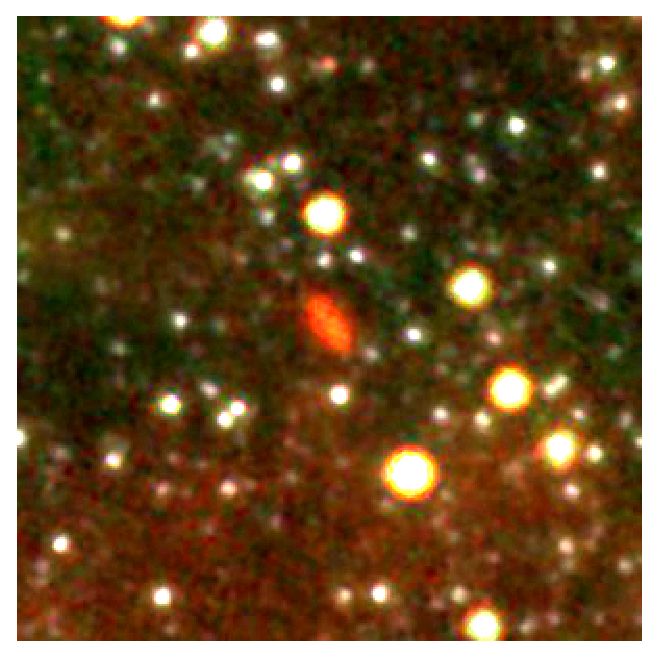
\includegraphics[width=0.19\textwidth]{./figures/3col/1.eps}}
\subfigure[Candidate 2]{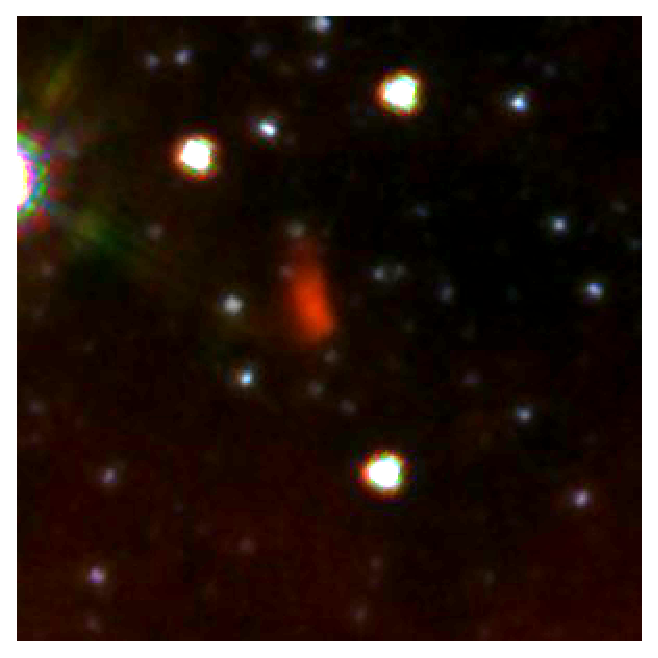
\includegraphics[width=0.19\textwidth]{./figures/3col/2.eps}}
\subfigure[Candidate 3]{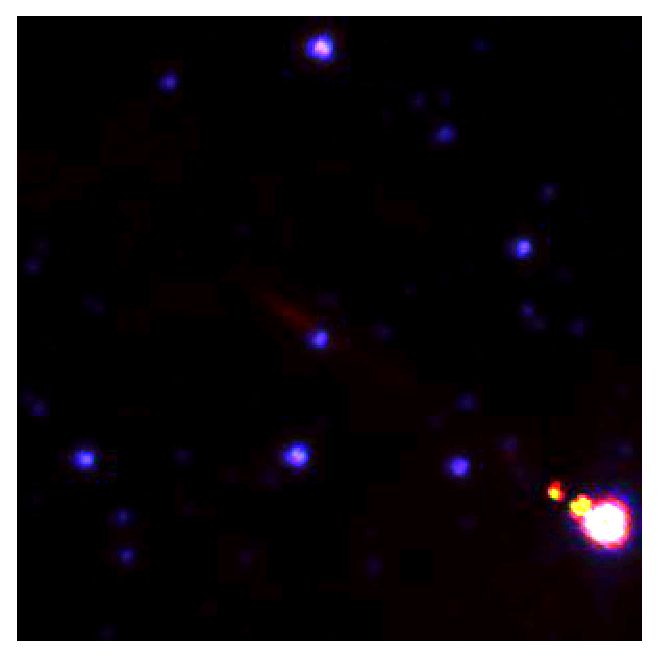
\includegraphics[width=0.19\textwidth]{./figures/3col/3.eps}}
\subfigure[Candidate 4]{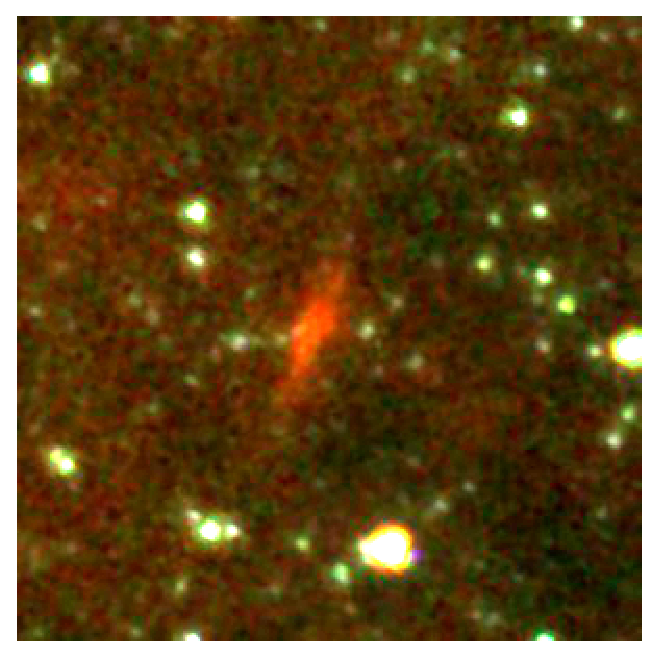
\includegraphics[width=0.19\textwidth]{./figures/3col/4.eps}}
\subfigure[Candidate 5]{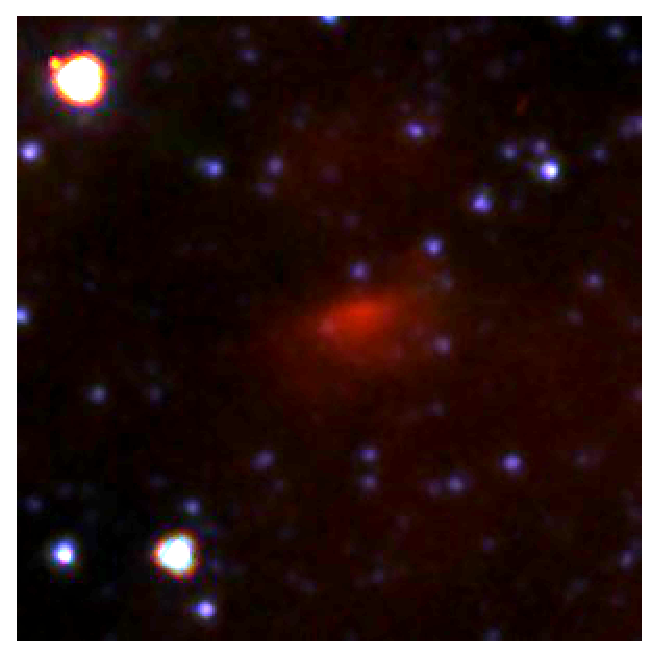
\includegraphics[width=0.19\textwidth]{./figures/3col/5.eps}}
\subfigure[Candidate 6]{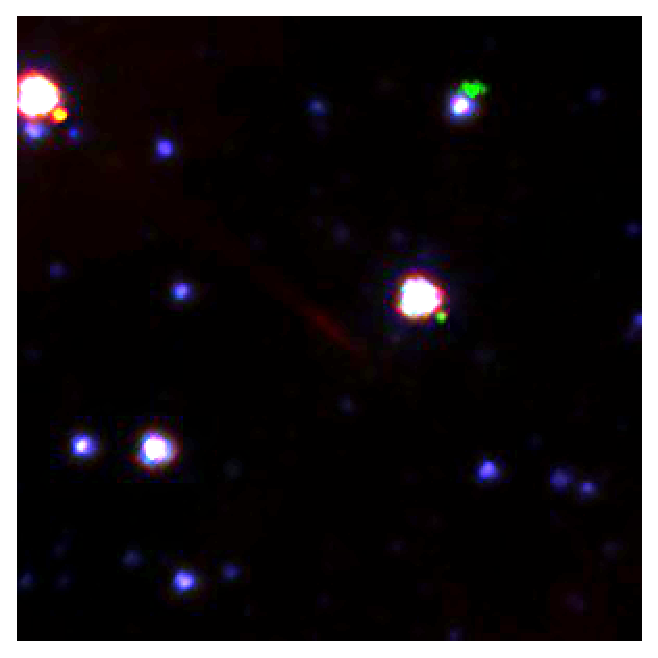
\includegraphics[width=0.19\textwidth]{./figures/3col/6.eps}}
\subfigure[Candidate 7]{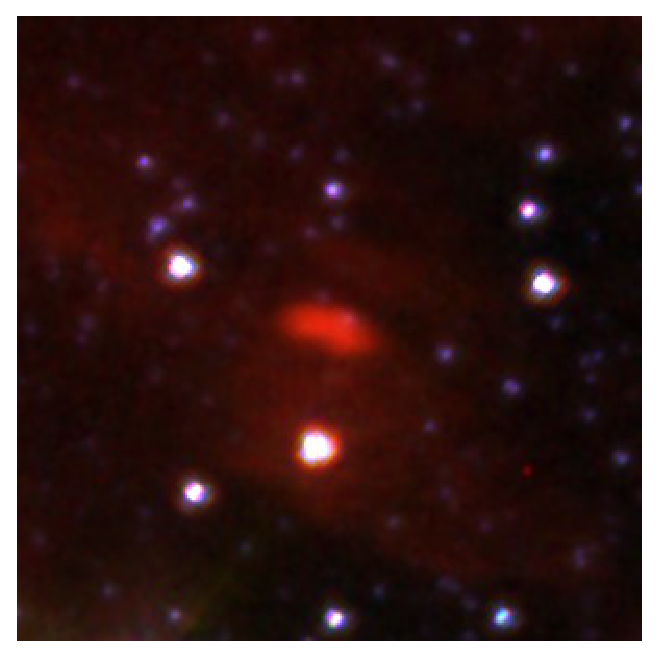
\includegraphics[width=0.19\textwidth]{./figures/3col/7.eps}}
\subfigure[Candidate 8]{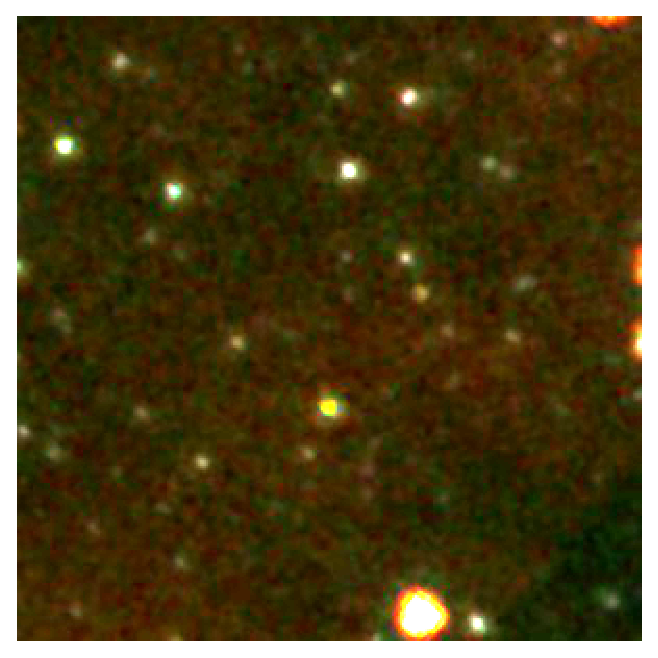
\includegraphics[width=0.19\textwidth]{./figures/3col/8.eps}}
\subfigure[Candidate 9]{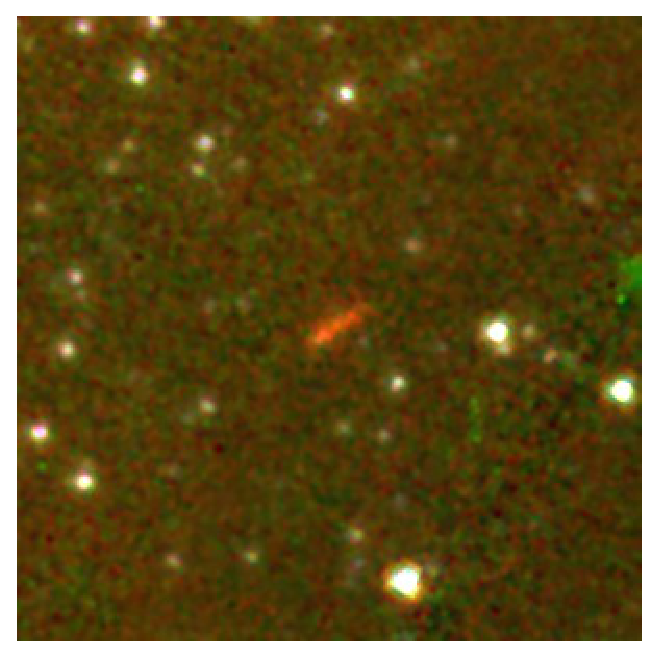
\includegraphics[width=0.19\textwidth]{./figures/3col/9.eps}}
\subfigure[Candidate 10]{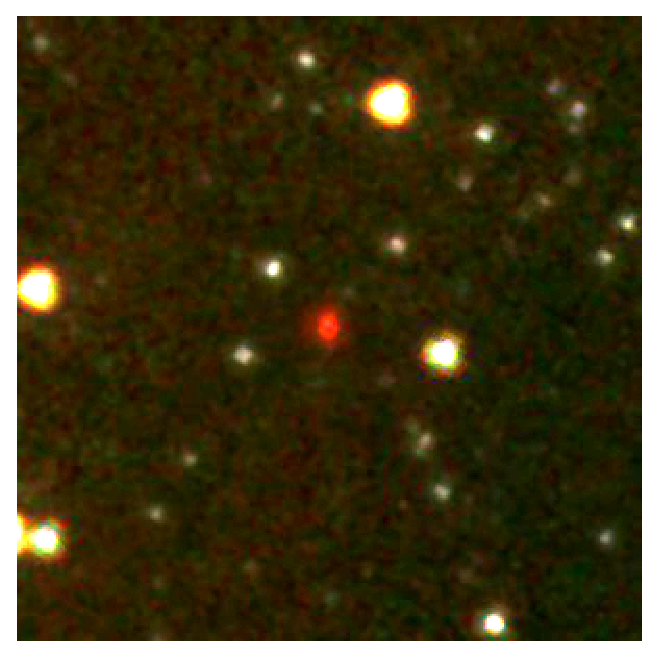
\includegraphics[width=0.19\textwidth]{./figures/3col/10.eps}}
\subfigure[Candidate 11]{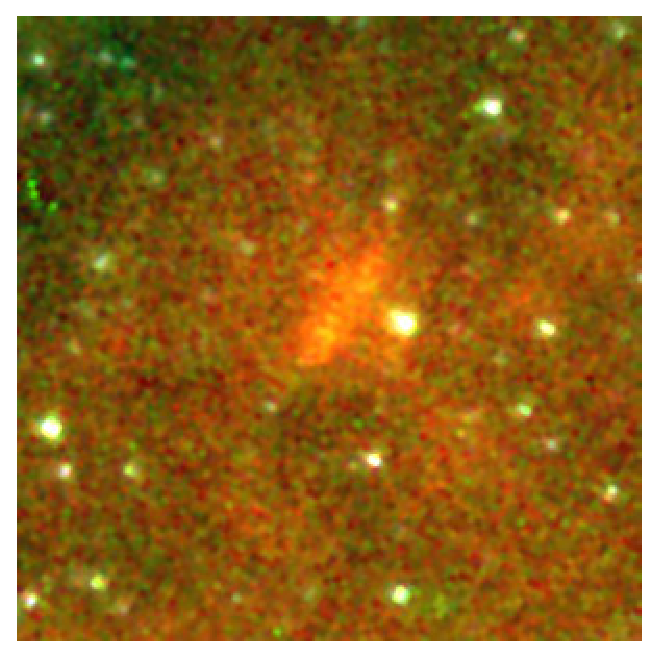
\includegraphics[width=0.19\textwidth]{./figures/3col/11.eps}}
\subfigure[Candidate 12]{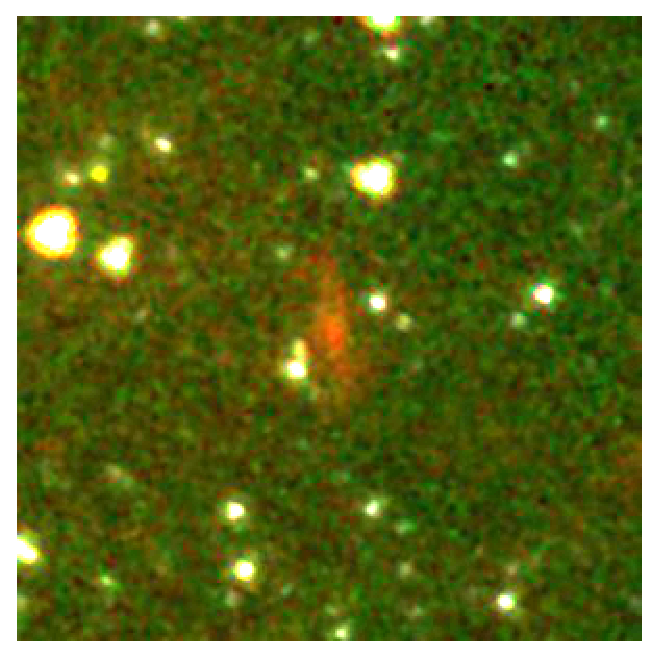
\includegraphics[width=0.19\textwidth]{./figures/3col/12.eps}}
\subfigure[Candidate 13]{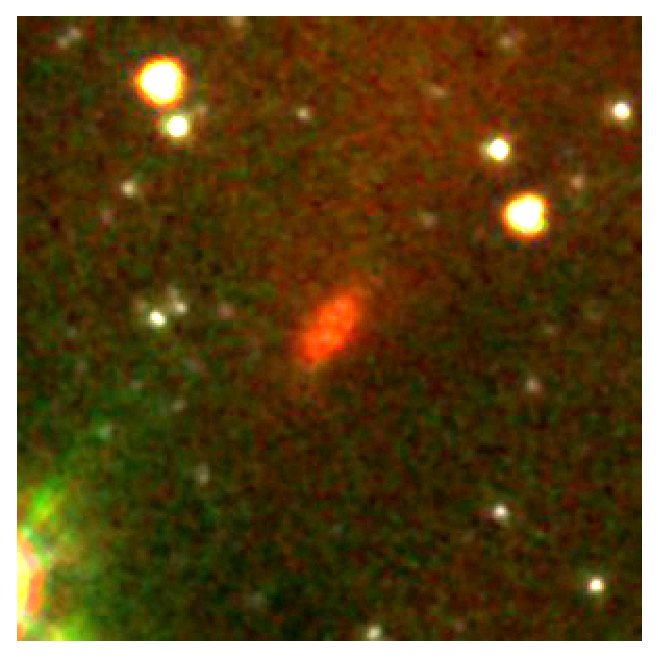
\includegraphics[width=0.19\textwidth]{./figures/3col/13.eps}}
\subfigure[Candidate 14]{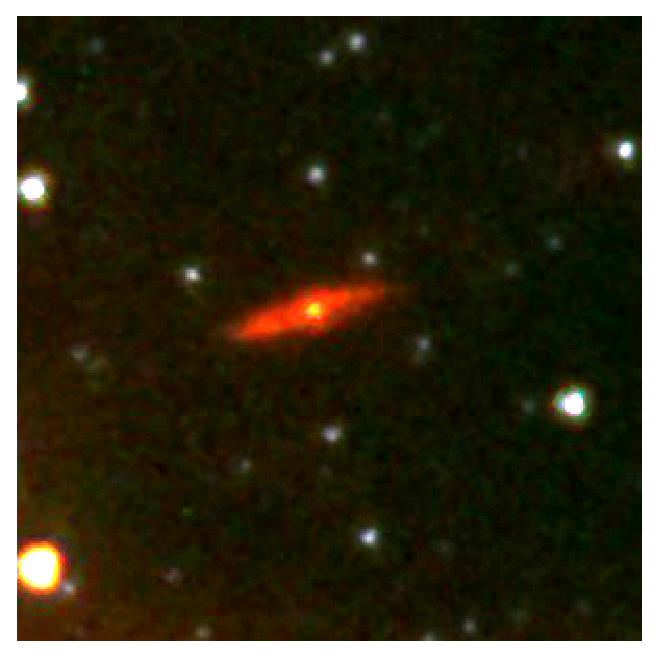
\includegraphics[width=0.19\textwidth]{./figures/3col/14.eps}}
\subfigure[Candidate 15]{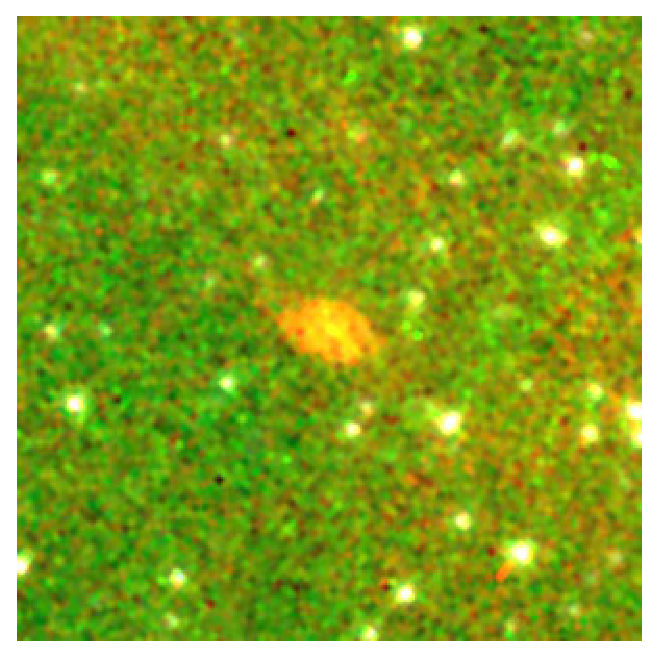
\includegraphics[width=0.19\textwidth]{./figures/3col/15.eps}}
\subfigure[Candidate 16]{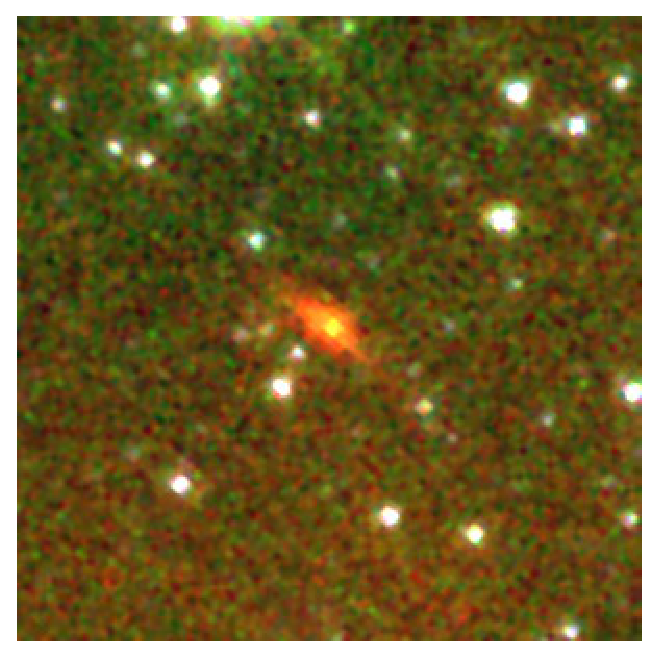
\includegraphics[width=0.19\textwidth]{./figures/3col/16.eps}}
\subfigure[Candidate 17]{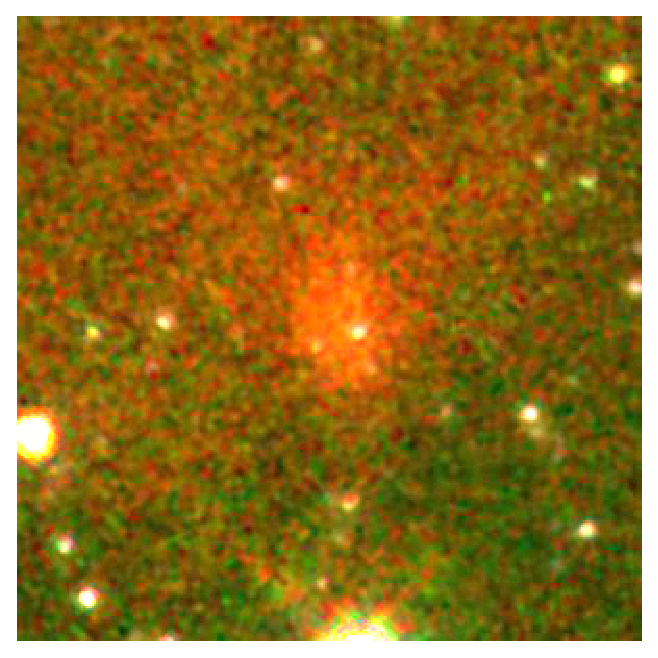
\includegraphics[width=0.19\textwidth]{./figures/3col/17.eps}}
\subfigure[Candidate 18]{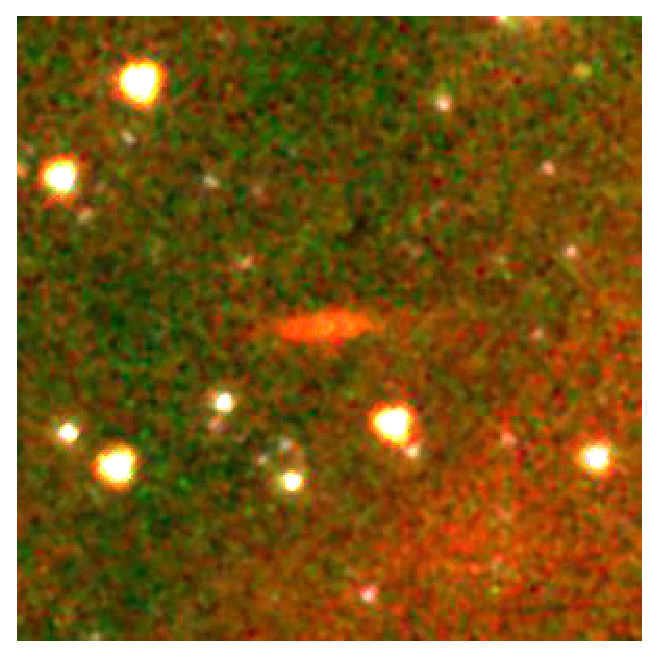
\includegraphics[width=0.19\textwidth]{./figures/3col/18.eps}}
\subfigure[Candidate 19]{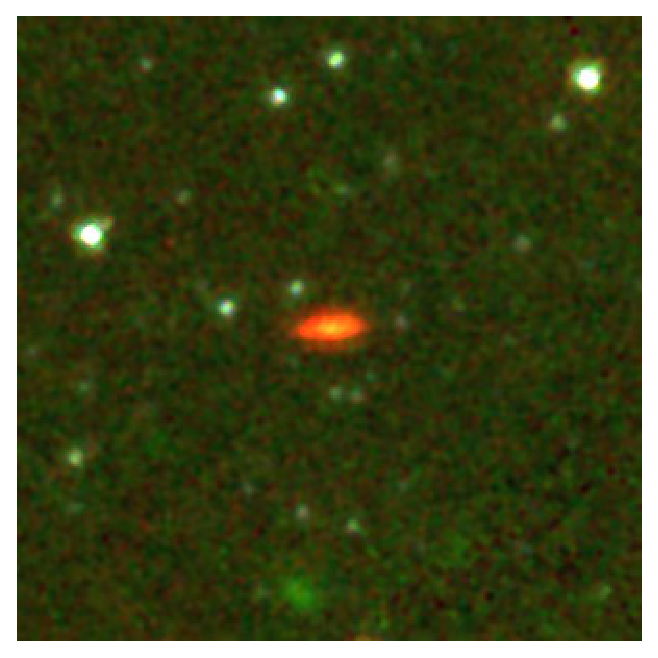
\includegraphics[width=0.19\textwidth]{./figures/3col/19.eps}}
\subfigure[Candidate 20]{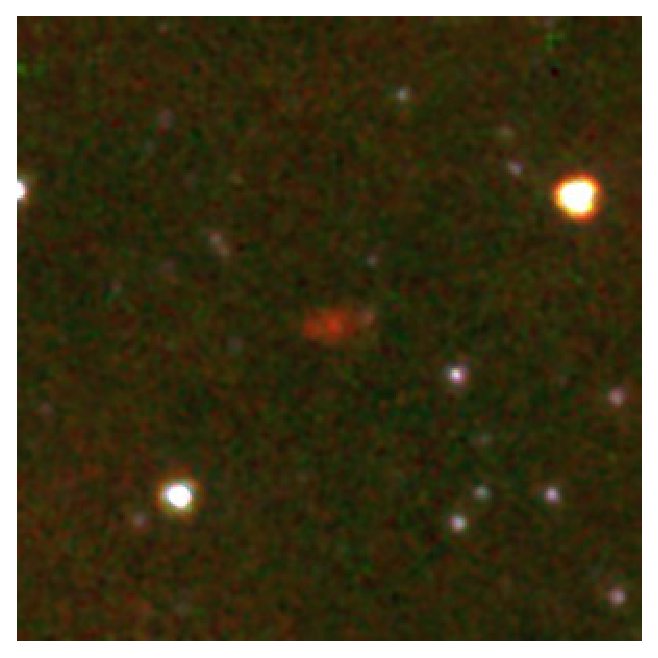
\includegraphics[width=0.19\textwidth]{./figures/3col/20.eps}}
\caption{Three-colour composite images of candidate galaxies 1--20, with RGB channels using Spitzer IRAC bands 8$\mu$m, 4.5$\mu$m and 3.6$\mu$m respectively.}
\label{gallery1}
\end{center}
\end{figure*} 

\begin{figure*}
\begin{center}
\subfigure[Candidate 21]{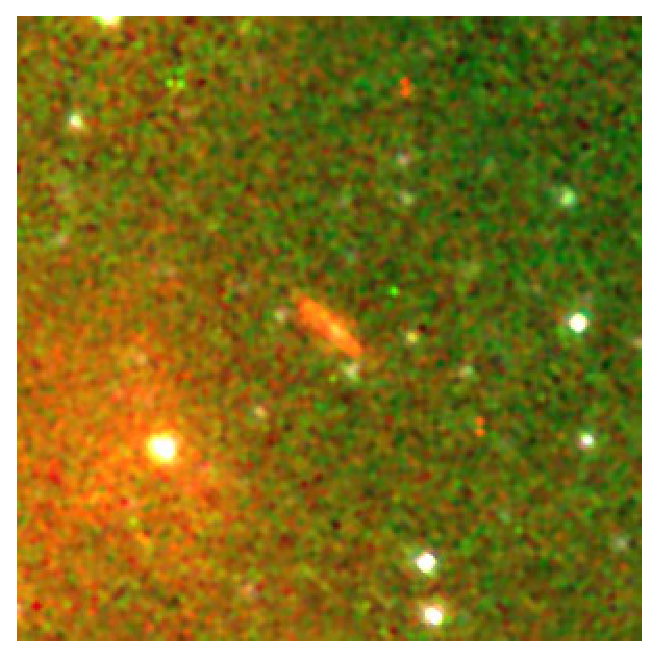
\includegraphics[width=0.19\textwidth]{./figures/3col/21.eps}}
\subfigure[Candidate 22]{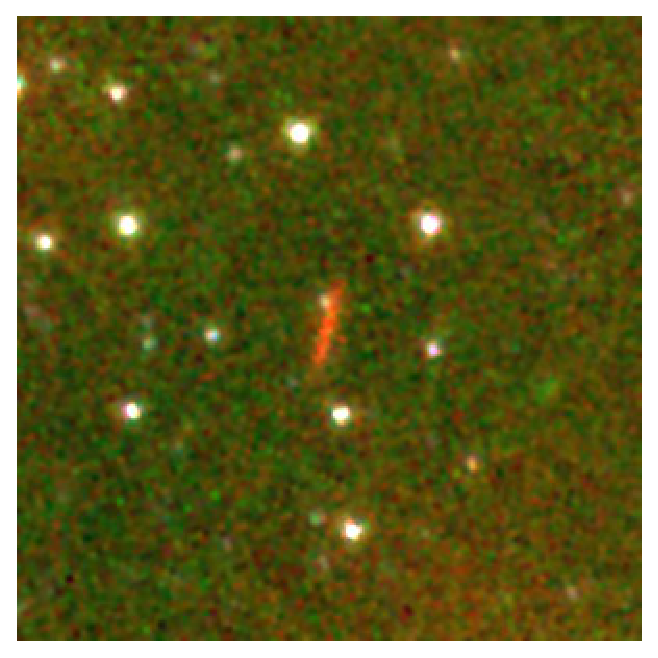
\includegraphics[width=0.19\textwidth]{./figures/3col/22.eps}}
\subfigure[Candidate 23]{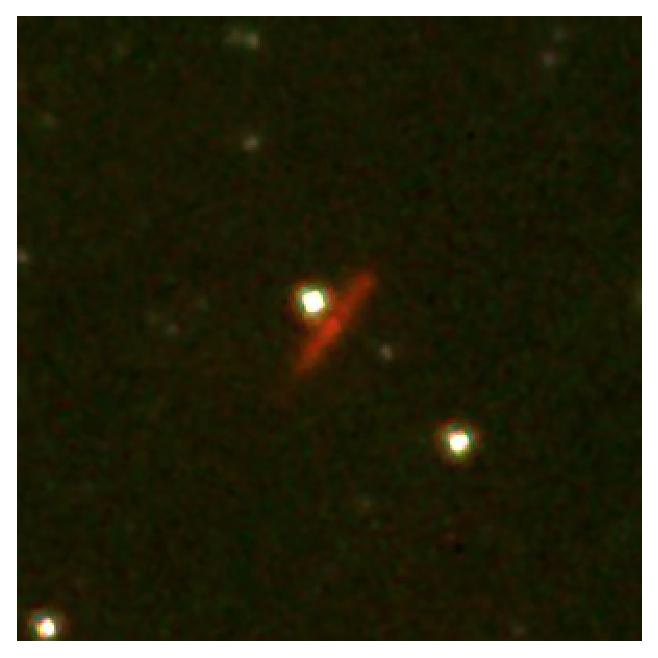
\includegraphics[width=0.19\textwidth]{./figures/3col/23.eps}}
\subfigure[Candidate 24]{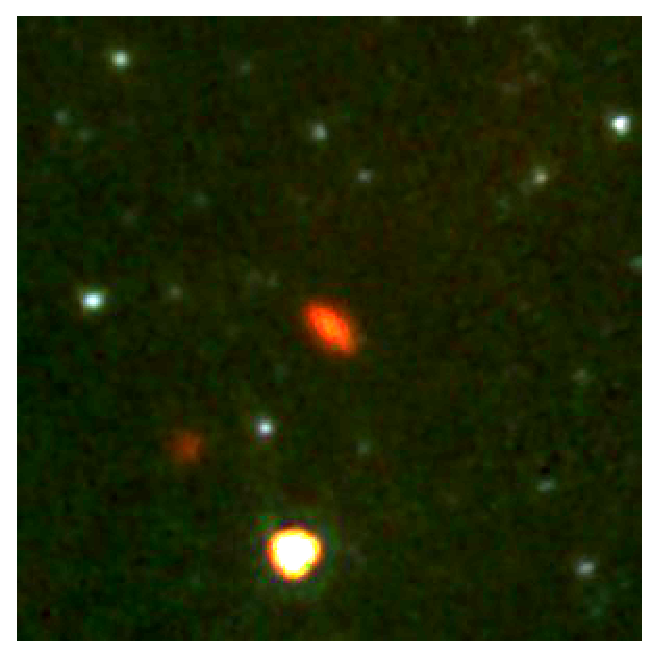
\includegraphics[width=0.19\textwidth]{./figures/3col/24.eps}}
\subfigure[Candidate 25]{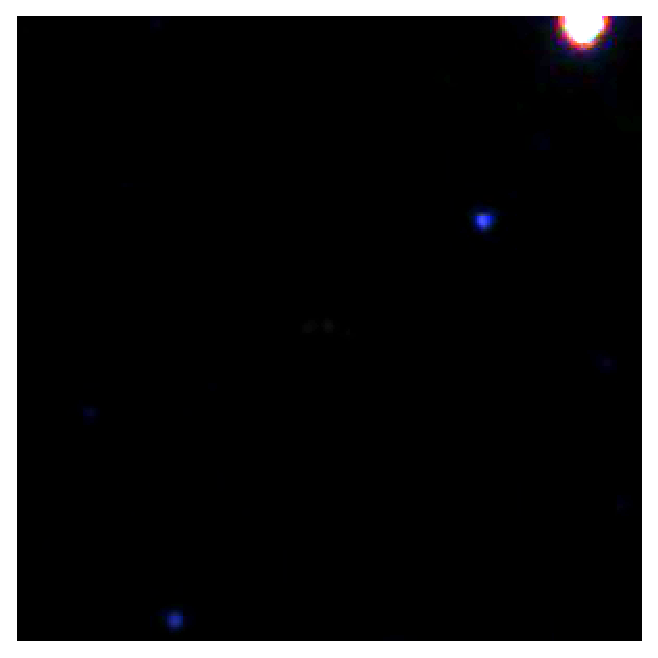
\includegraphics[width=0.19\textwidth]{./figures/3col/25.eps}}
\subfigure[Candidate 26]{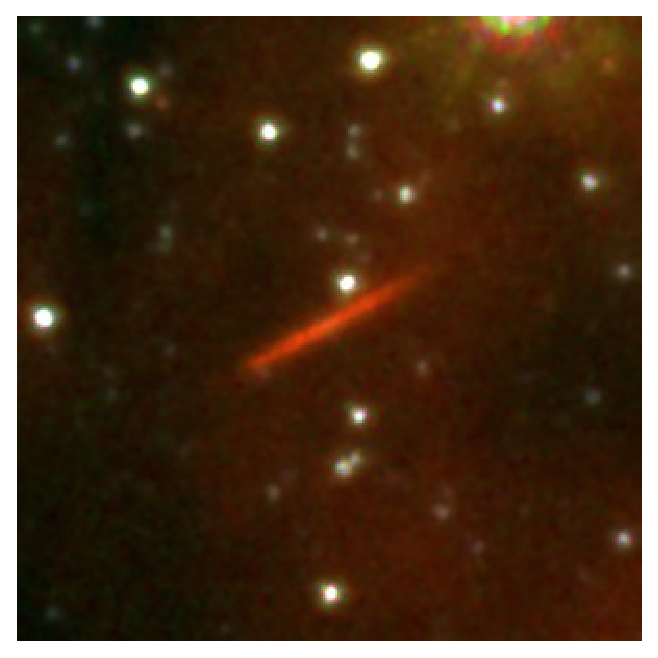
\includegraphics[width=0.19\textwidth]{./figures/3col/26.eps}}
\subfigure[Candidate 27]{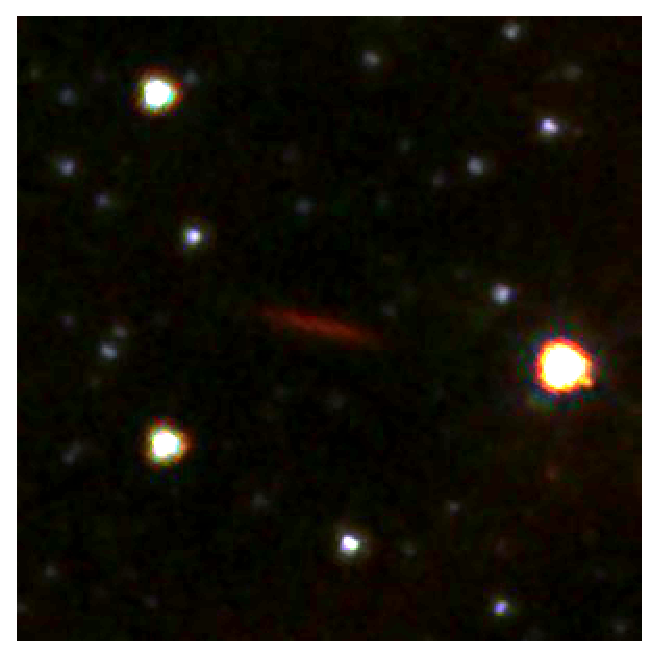
\includegraphics[width=0.19\textwidth]{./figures/3col/27.eps}}
\subfigure[Candidate 28]{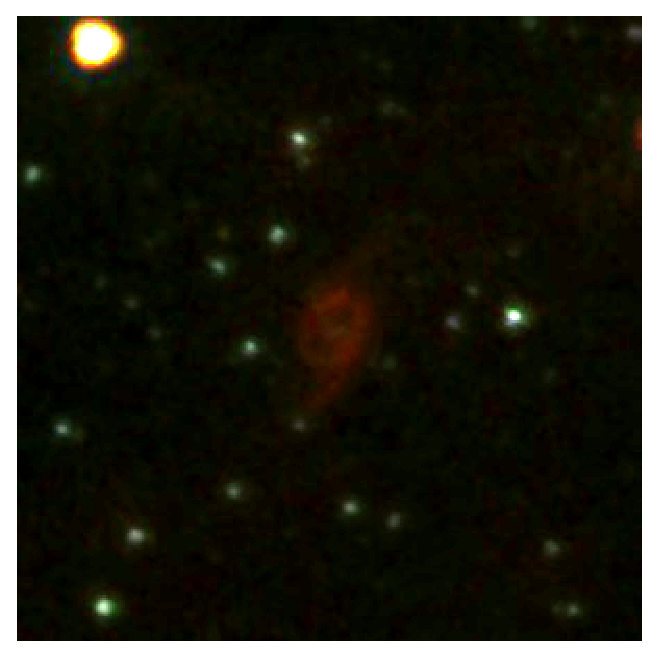
\includegraphics[width=0.19\textwidth]{./figures/3col/28.eps}}
\subfigure[Candidate 29]{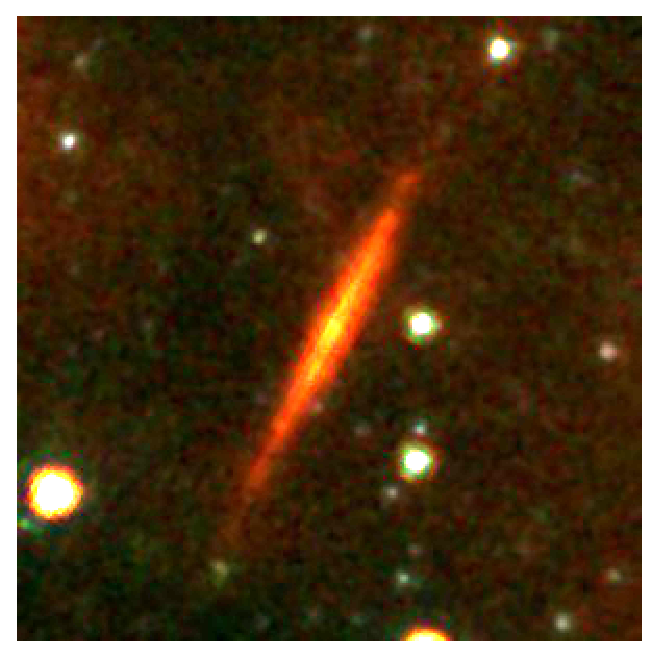
\includegraphics[width=0.19\textwidth]{./figures/3col/29.eps}}
\subfigure[Candidate 30]{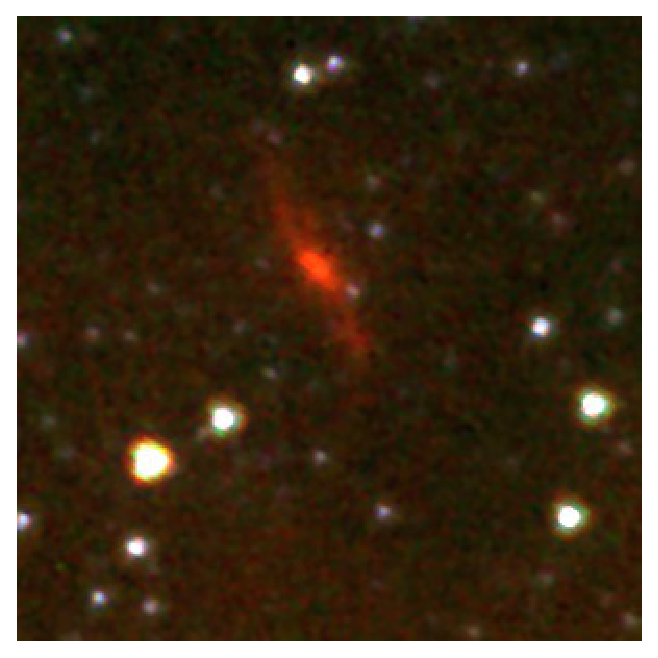
\includegraphics[width=0.19\textwidth]{./figures/3col/30.eps}}
\subfigure[Candidate 31]{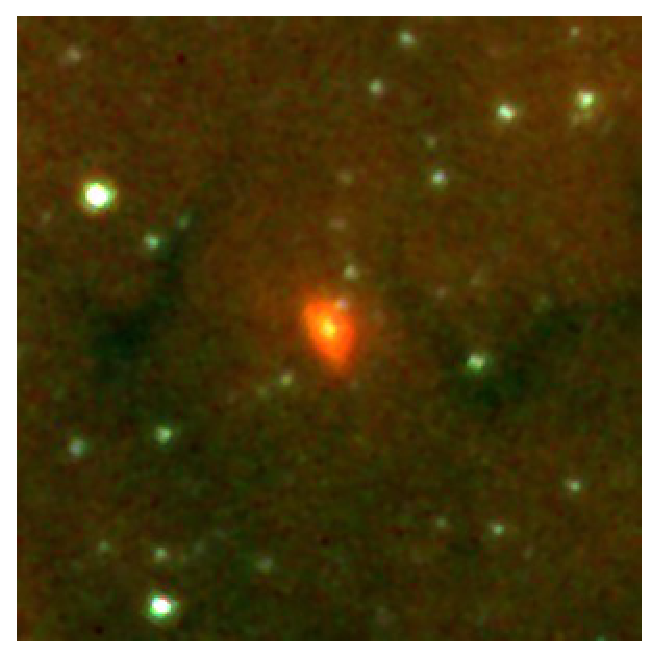
\includegraphics[width=0.19\textwidth]{./figures/3col/31.eps}}
\subfigure[Candidate 32]{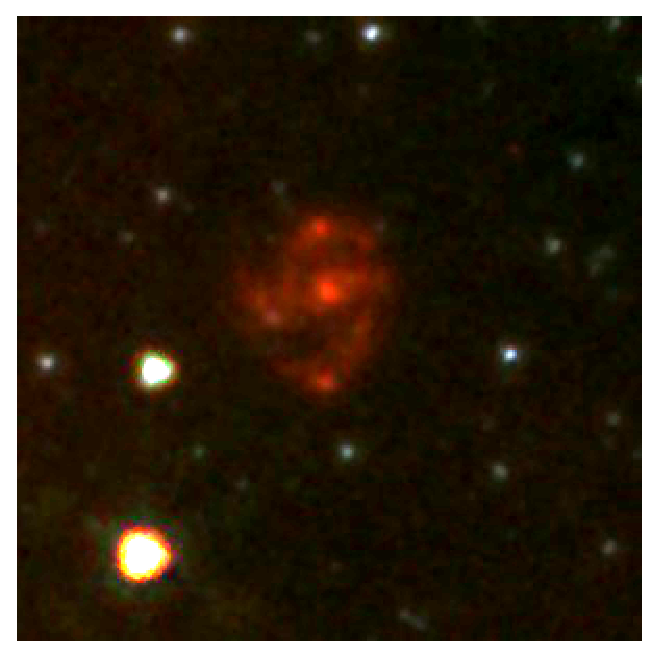
\includegraphics[width=0.19\textwidth]{./figures/3col/32.eps}}
\subfigure[Candidate 33]{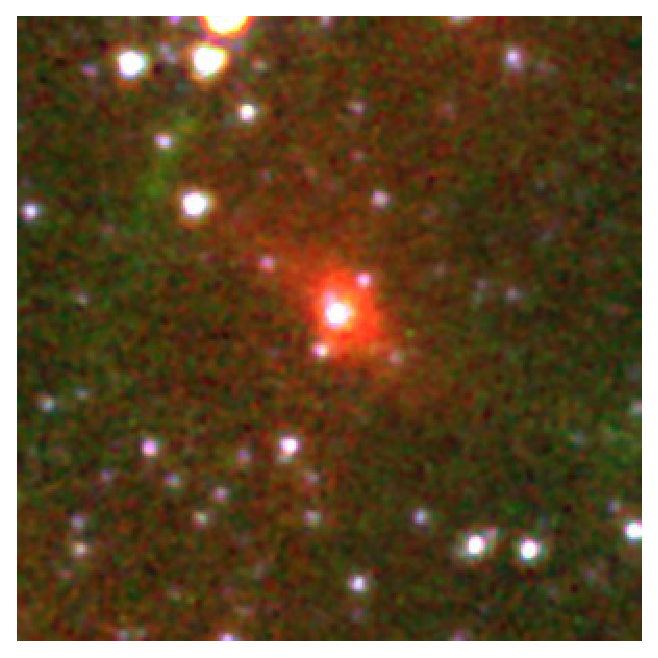
\includegraphics[width=0.19\textwidth]{./figures/3col/33.eps}}
\subfigure[Candidate 34]{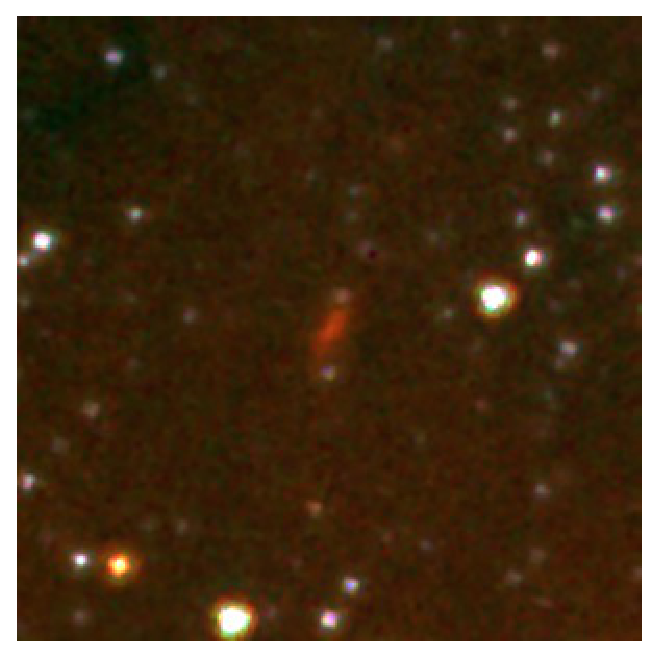
\includegraphics[width=0.19\textwidth]{./figures/3col/34.eps}}
\subfigure[Candidate 35]{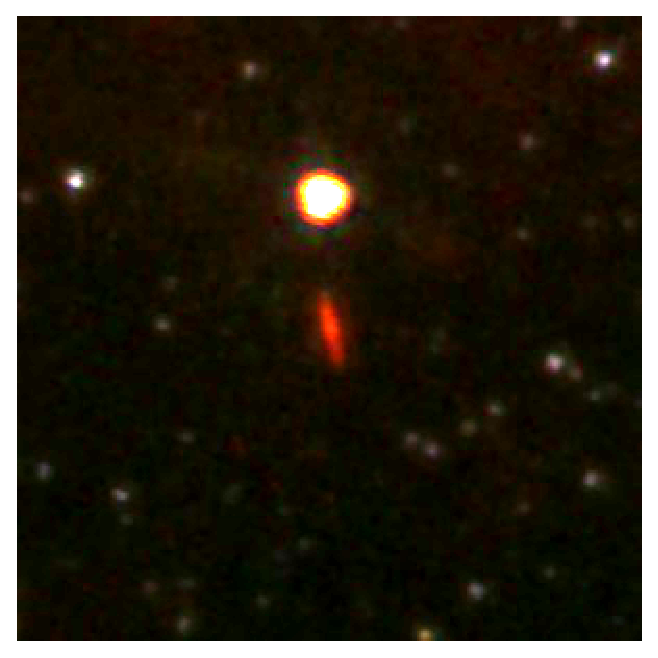
\includegraphics[width=0.19\textwidth]{./figures/3col/35.eps}}
\subfigure[Candidate 36]{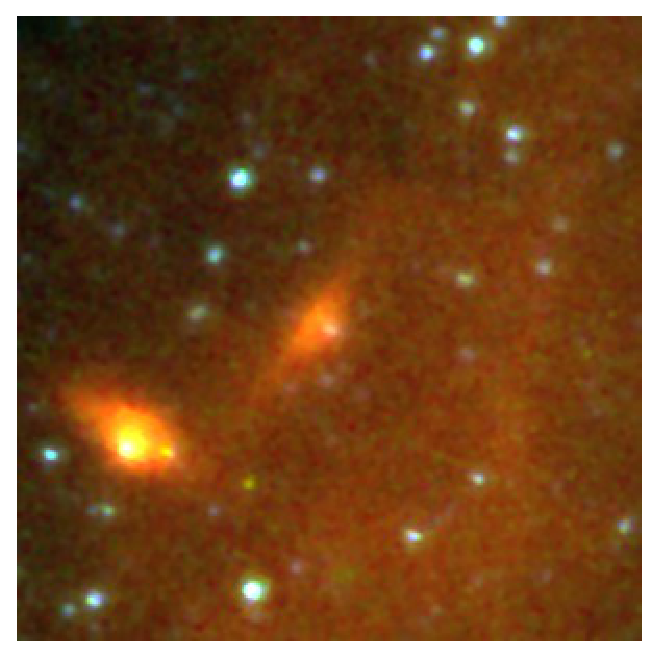
\includegraphics[width=0.19\textwidth]{./figures/3col/36.eps}}
\subfigure[Candidate 37]{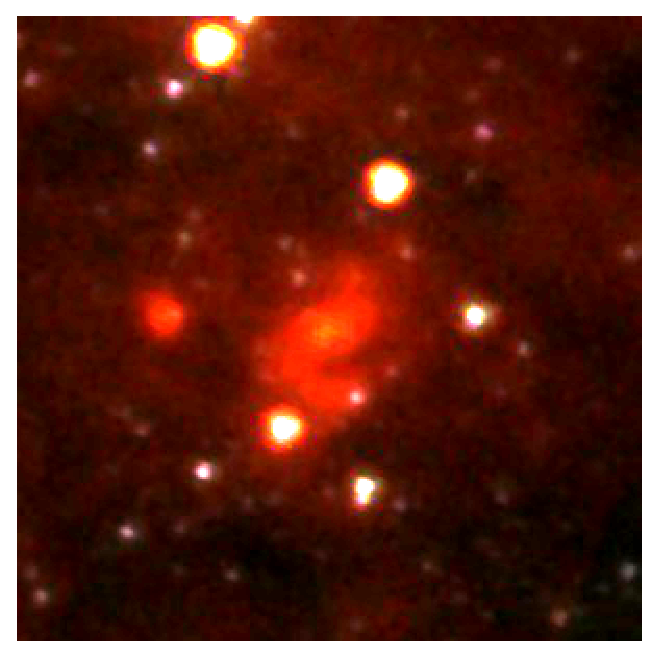
\includegraphics[width=0.19\textwidth]{./figures/3col/37.eps}}
\subfigure[Candidate 38]{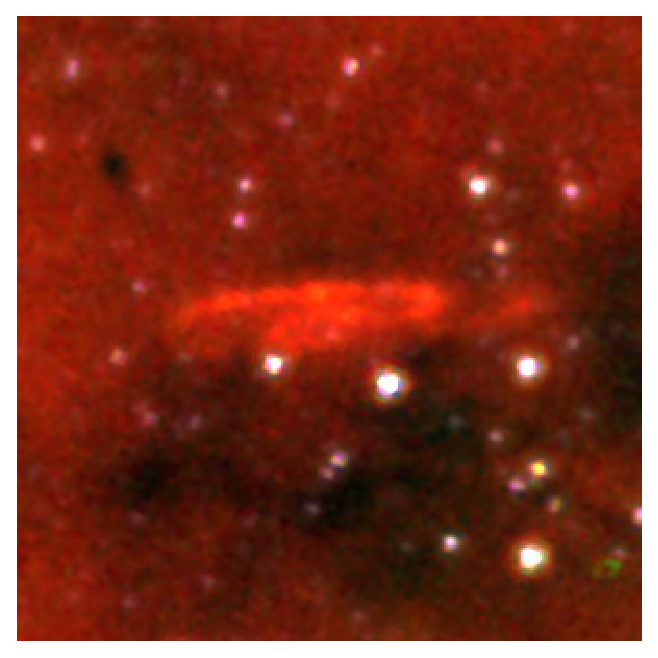
\includegraphics[width=0.19\textwidth]{./figures/3col/38.eps}}
\subfigure[Candidate 39]{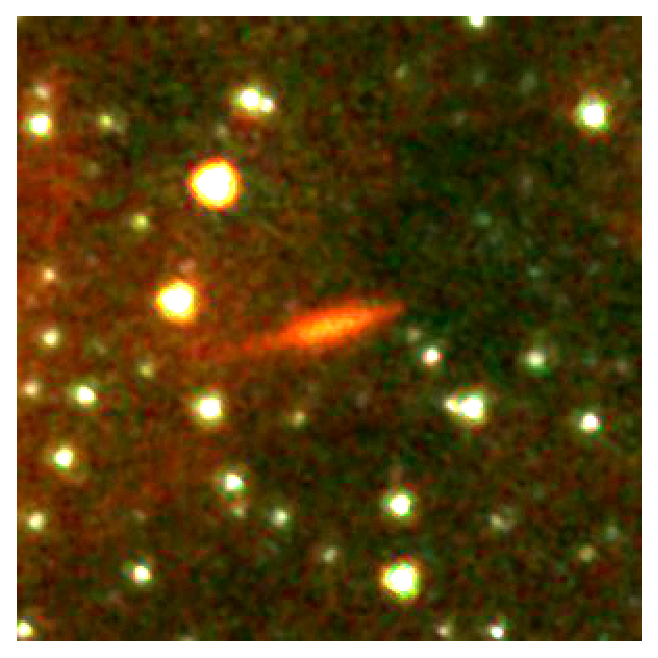
\includegraphics[width=0.19\textwidth]{./figures/3col/39.eps}}
\subfigure[Candidate 40]{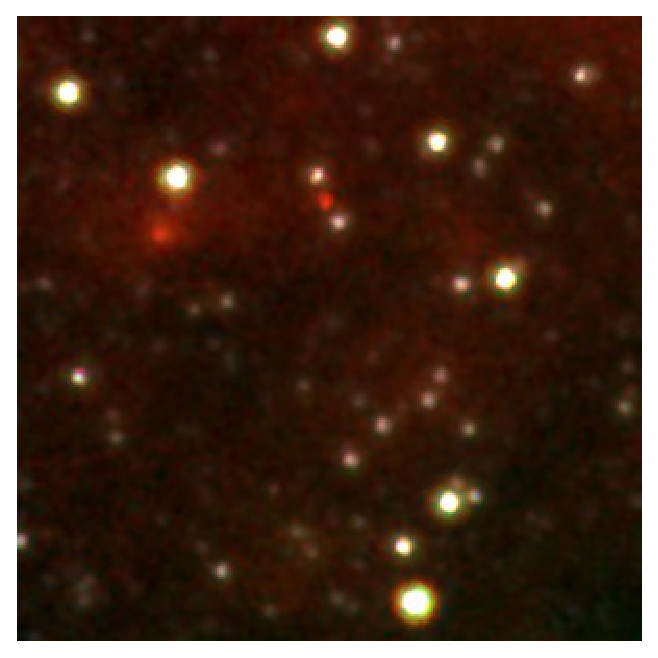
\includegraphics[width=0.19\textwidth]{./figures/3col/40.eps}}
\subfigure[Candidate 41]{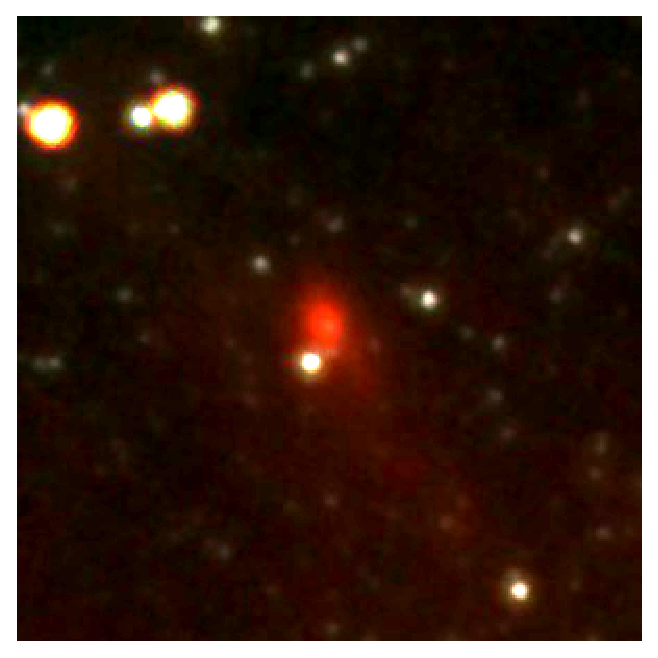
\includegraphics[width=0.19\textwidth]{./figures/3col/41.eps}}
\subfigure[Candidate 42]{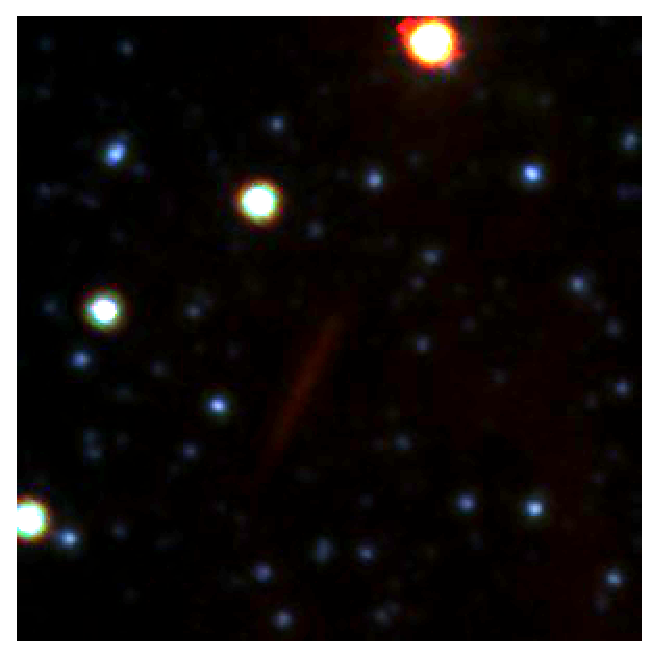
\includegraphics[width=0.19\textwidth]{./figures/3col/42.eps}}
\subfigure[Candidate 43]{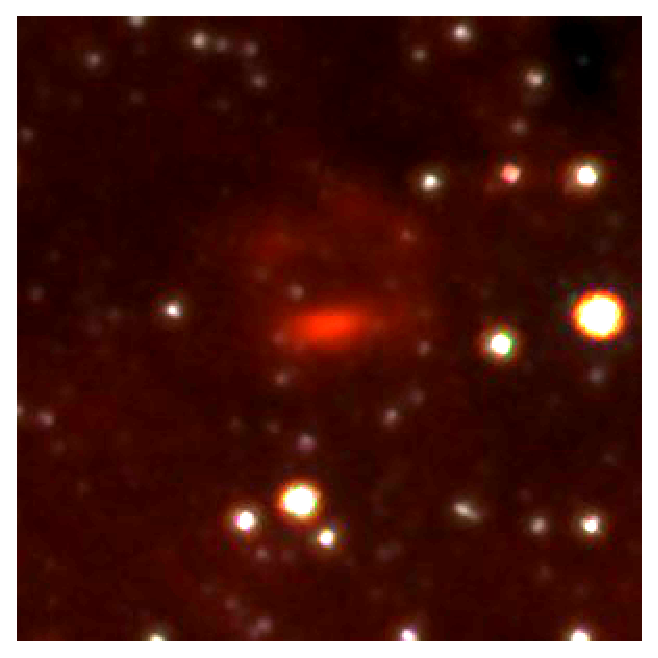
\includegraphics[width=0.19\textwidth]{./figures/3col/43.eps}}
\caption{Three-colour composite images of candidate galaxies 21--43, with RGB channels using Spitzer IRAC bands 8$\mu$m, 4.5$\mu$m and 3.6$\mu$m respectively.}
\label{gallery2}
\end{center}
\end{figure*} 

\subsection{Galaxy catalogue}

\section{Results}

\subsection{Spectral energy distributions}

\subsection{Comparison with large-scale structure from 2MASS}

\begin{figure}
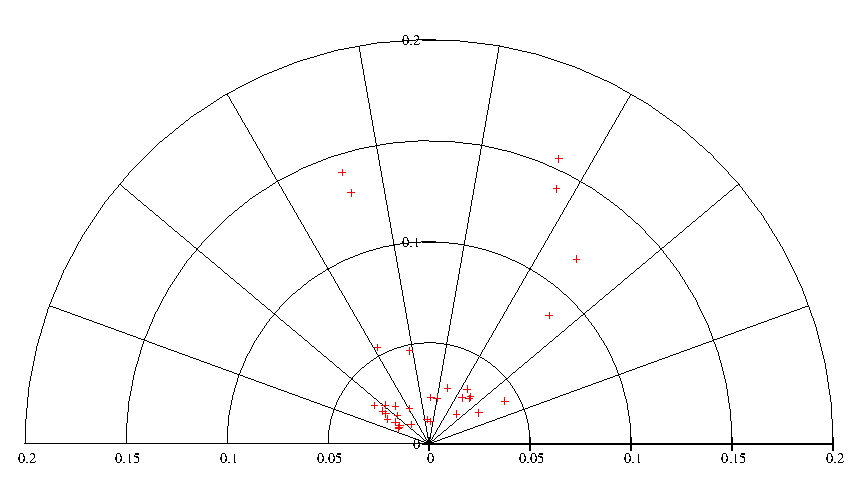
\includegraphics[width=0.48\textwidth]{./figures/polar.eps}
\caption{Positions of galaxies relative to our own.}
\label{polar}
\end{figure}

\begin{figure}
\includegraphics[width=0.48\textwidth]{./figures/2MRS_latlon.eps}
\caption{Positions of galaxies relative to our own.}
\label{2mrs}
\end{figure}

\begin{figure}
\includegraphics[width=0.48\textwidth]{./figures/2MRS_zlon.eps}
\caption{Positions of galaxies relative to our own.}
\label{2mrsz}
\end{figure}

\begin{figure}
\includegraphics[width=0.48\textwidth]{./figures/2MRS_zlat.eps}
\caption{Positions of galaxies relative to our own.}
\label{2mrsz2}
\end{figure}

\begin{figure*}
\includegraphics[width=0.98\textwidth]{./figures/2MRS_All.eps}
\caption{Positions of galaxies relative to our own.}
\label{2mrs_all}
\end{figure*}

\section{Discussion}

\section{Summary and future work}

\section*{Acknowledgments}

This publication has been made possible by the participation of more than 40,000 volunteers on the Milky Way Project. Their contributions are acknowledged individually at http://www.milkywayproject.org/authors. The Milky Way Project, and R.J.S. were supported by The Leverhulme Trust. The `Talk' discussion tool used in the MWP was developed at the Adler Planetarium with support from the National Science Foundation CDI grant : DRL-0941610. 

This work is based on observations made with the Spitzer Space Telescope, which is operated by the Jet Propulsion Laboratory, California Institute of Technology under a contract with NASA. This research has made use of the SIMBAD database, operated at CDS, Strasbourg, France.

\bibliographystyle{apj}
\bibliography{mwpref}

\clearpage

\appendix{Galaxy Images and SEDs}

\begin{figure*}
\begin{center}
\subfigure[]{
\includegraphics[width=0.22\textwidth]{./figures/cutouts/1.eps}}
\subfigure[]{\includegraphics[width=0.22\textwidth]{./figures/IRAC4/1.eps}}
\subfigure[]{\includegraphics[width=0.22\textwidth]{./figures/3col/1.eps}}
\subfigure[]{\includegraphics[width=0.32\textwidth]{./figures/seds/gal1.eps}}
\caption{Data for galaxy candidate 1. Subfigures show (a) MWP image cutout; (b) IRAC 8$\mu$m data; (c) Three-colour composite with RGB channels using Spitzer IRAC bands 8$\mu$m, 4.5$\mu$m and 3.6$\mu$m respectively; and (d) measured SED for this object.}
\label{gal1}
\end{center}
\end{figure*} 

\begin{figure*}
\begin{center}
\subfigure[]{\includegraphics[width=0.22\textwidth]{./figures/cutouts/2.eps}}
\subfigure[]{\includegraphics[width=0.22\textwidth]{./figures/IRAC4/2.eps}}
\subfigure[]{\includegraphics[width=0.22\textwidth]{./figures/3col/2.eps}}
\subfigure[]{\includegraphics[width=0.32\textwidth]{./figures/seds/gal2.eps}}
\caption{Data for galaxy candidate 2. Subfigures show (a) MWP image cutout; (b) IRAC 8$\mu$m data; (c) Three-colour composite with RGB channels using Spitzer IRAC bands 8$\mu$m, 4.5$\mu$m and 3.6$\mu$m respectively; and (d) measured SED for this object.}
\label{gal2}
\end{center}
\end{figure*} 


\end{document}

